%%%%%%%%%%%%%%%%%%%%%%%%%%%%%%%%%%%%%%%%%
% Beamer Presentation
% LaTeX Template
% Version 1.0 (10/11/12)
%
% This template has been downloaded from:
% http://www.LaTeXTemplates.com
%
% License:
% CC BY-NC-SA 3.0 (http://creativecommons.org/licenses/by-nc-sa/3.0/)
%
%%%%%%%%%%%%%%%%%%%%%%%%%%%%%%%%%%%%%%%%%

%----------------------------------------------------------------------------------------
%	PACKAGES AND THEMES
%---------------------------------------------------------------------------------------

\documentclass{beamer}
\usepackage[spanish]{babel}
 \usepackage{algpseudocode}
\usepackage[utf8]{inputenc}
\mode<presentation> {


\usetheme{PaloAlto}

}

\usepackage{graphicx} % Allows including images


%----------------------------------------------------------------------------------------
%	TITLE PAGE
%----------------------------------------------------------------------------------------

\title[Práctica 4]{Cena de gala} % The short title appears at the bottom of every slide, the full title is only on the title page

\author{Algorítmica} % Your name
\institute[UGR] % Your institution as it will appear on the bottom of every slide, may be shorthand to save space
{
Universidad de Granada \\ % Your institution for the title page
\medskip

}
\date{\today} % Date, can be changed to a custom date

\begin{document}

\begin{frame}
\titlepage % Print the title page as the first slide
\end{frame}

\begin{frame}
\frametitle{Índice} % Table of contents slide, comment this block out to remove it
\tableofcontents % Throughout your presentation, if you choose to use \section{} and \subsection{} commands, these will automatically be printed on this slide as an overview of your presentation
\end{frame}

%----------------------------------------------------------------------------------------
%	PRESENTATION SLIDES
%----------------------------------------------------------------------------------------

\section{Introducción }
\begin{frame}
	\frametitle{Introducción}
	\begin{itemize}
		\item El objetivo de esta práctica es diseñar un algoritmo Backtracking, que resuelva uno de los cinco problemas de la práctica y realizar un estudio empírico de su eficiencia.
	\end{itemize}
\end{frame}


%------------------------------------------------
\section{Ejercicio} 
\begin{frame}
	\frametitle{Enunciado del ejercicio}
	Se desea sentar a N invitados alrededor de una mesa, de manera que cada invitado tendrá a su lado a otros dos. Cada par de invitados tiene un nivel de compatibilidad. Se desea maximizar la compatibilidad de estos comensales.
	
\end{frame}

%------------------------------------------------
\section{Diseño del algoritmo} 
\begin{frame}
	\frametitle{Diseño del algoritmo}
	\begin{itemize}
		\item \textbf{Solución parcial}: Solución parcial al problema de tamaño menor que N. (Conjunto \textbf{Sp})
		\item \textbf{Restricciones explícitas}: Los valores que puede tomar la solución son los enteros de 1 a N. Donde N es el número total de invitados.  
		\item \textbf{Restricciones implícitas}: Estas restricciones son las que determinan si una función parcial puede llevarnos a una solución del problema.
	\end{itemize}
	
\end{frame}


\begin{frame}
		\frametitle{Diseño del algoritmo}
	Dada una matriz M[i][j] 
	Mantenemos en la matriz la afinidad  entre 
	el comensal i y el comensal j
	

\[ \left( \begin{array}{ccc}
0 & 30 & 15 \\
30 & 0 & 20 \\
15 & 20 & 0 \end{array} \right)\] 
\end{frame}

\section{Pseudocódigo}

\begin{frame}
		\frametitle{Pseudocódigo}
		\footnotesize{	
		\begin{algorithmic}				
			\Require Matriz, S\_final[N] S\_parcial[N] Sentados[N]={false} comensal\_actual, nivel,valor\_maximo=0;
			\State \textbf{Funcion(S,S\_parcial,Sentados,comensal\_actual,nivel):}
				\State Sentados[comensal\_actual]=true;
				\State	   S\_parcial[nivel - 1]=comensal\_actual;
			\For {\textbf{i} to \textbf{N}}
	
			\If {Sentados[i]==false}
				\State 	valor\_actual = CalcularSolucionActual(S\_parcial);
				\State 	\textbf{Funcion(S,S\_parcial,Sentados,i,nivel+1);}
				\If{nodo\_actual == nodo\_hoja}
					\State{ valor\_actual = CalcularSolucionActual()}
					\If{valor\_actual \textbf{mayor que} valor\_maximo)}
						\State{ S\_final = S\_Actual}
						\State{ valor\_maximo = valor\_actual}
					\EndIf
				\EndIf
				
				\State Sentados[i] = false;
				\EndIf
				\EndFor
				
				
			\end{algorithmic}	
		}
\end{frame}

\section{Eficiencia}


\begin{frame}
	\frametitle{Eficiencia Empírica}	
	
	\begin{figure}[H]
		\centering
		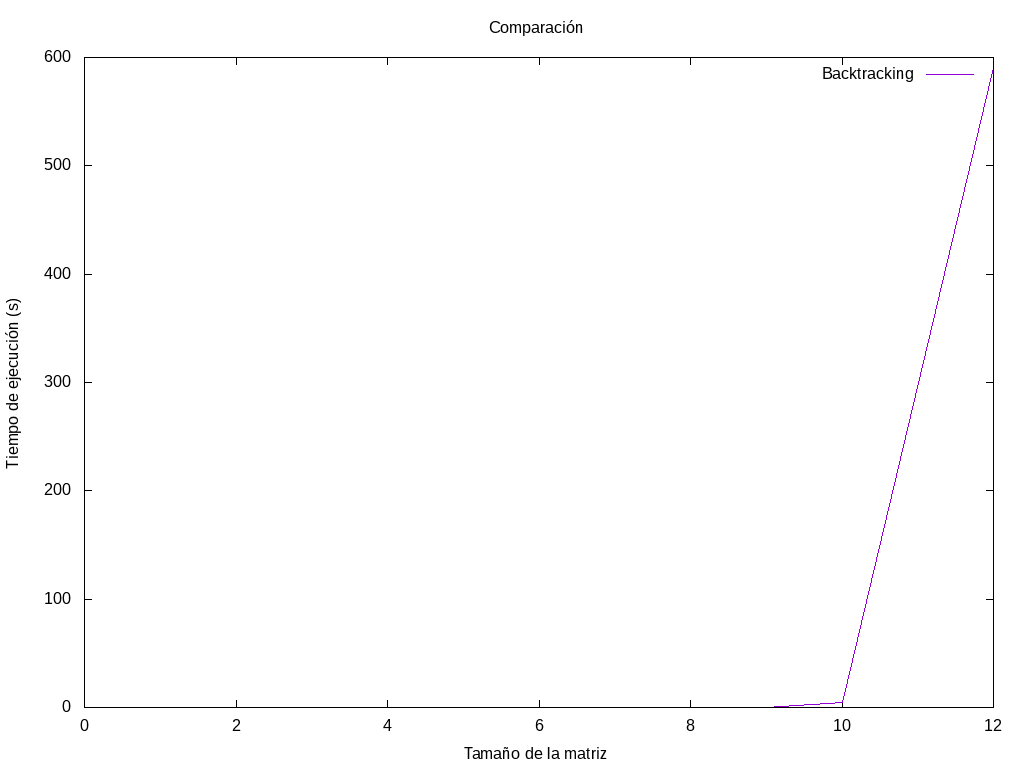
\includegraphics[width=0.7\linewidth,scale=1.5]{../Codigo/backtrackempirica}
		\caption{algoritmo backtracking}
		\label{fig:backtrackhibrida}
	\end{figure}
	
	
	
\end{frame}







\begin{frame}
	\frametitle{Eficiencia Híbrida}	

		\begin{figure}[H]
\centering
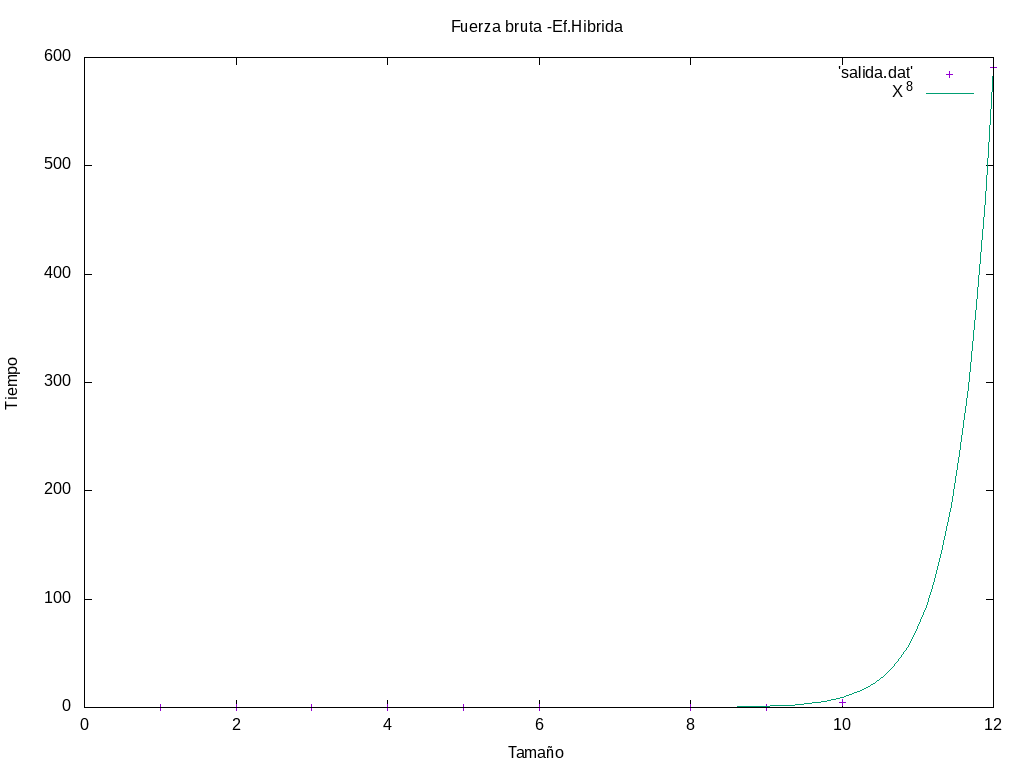
\includegraphics[width=0.7\linewidth,scale=1.5]{../Codigo/backtrackhibrida}
\caption{comparación x**8 vs algoritmo backtracking}
\label{fig:backtrackhibrida}
\end{figure}


	
\end{frame}

\begin{frame}
	\frametitle{Eficiencia Híbrida}	
	Ajuste con X**8

	\begin{table}[]
		\centering
		\caption{Ef híbrida obtenida}
		\label{my-label}
		\begin{tabular}{lllll}
			& Final set of parameters &   Asymptotic Standard Error & \\
			& a0  = 8.59555e-09 &  +/- 2.326e-11    (0.2706\%)&  \\
		
		\end{tabular}
	\end{table}
	
	
	
\end{frame}



\end{document} 
